\documentclass[UTF8,a4paper,12pt]{ctexart}
\usepackage{thesis-style}
\usepackage{amsmath}

\graphicspath{{../../outputs/experiment2/}}
\headermark{《金融经济数据挖掘》实验二报告}
\reporttitle{《金融经济数据挖掘》实验报告}
\reportsubtitle{实验二：基于市场情绪的金融羊群效应指数构建}
\author{丁致宇}
\studentid{202331060205}
\major{数据科学与大数据技术}
\phone{18765788600}
\date{2026年6月}

\begin{document}

\maketitle

\begin{ustcabstract}
本报告围绕《金融经济数据挖掘》实验二“金融非结构化数据情感分析”展开，基于实验一输出的周度情绪指标构建 H1、H2、H3 羊群效应指数。实验先按正面新闻占正负情绪新闻比例计算 $P_t$，再用过去 4 周 $P_t$ 均值作为正常情绪基准，得到情绪偏离度 $H1_t$；随后根据“观点是否一边倒”的金融逻辑构造分歧度 $H2_t$，最终合成周度羊群效应指数 $H3_t$。本次共读取 51 行周度情绪样本，剔除首期历史基准缺失后输出 50 行羊群效应指标，日期范围为 2014-10-20 至 2015-10-21。质量检查 6 项全部通过，最高羊群效应周出现在 2015-09-16，$H3_t=0.864687$。实验输出包括 CSV 指标表、SQLite 数据库、指标时序图、指标表截图、核心程序截图、AI 交互记录、AI 代码审查表和代码附录。
\end{ustcabstract}
\keywords{金融文本挖掘；市场情绪；羊群效应；Min-Max 归一化；SQLite；LaTeX 报告}

\clearpage
\tableofcontents
\clearpage

\section{实验要求理解}

实验二承接实验一输出的周度情绪指标，核心任务是将市场情绪进一步转化为可用于后续回归和机器学习建模的羊群效应指数。指导书要求用周度情绪构建 $H1$、$H2$、$H3$，对指标进行归一化处理，并输出包含交易日、$H1_t$、$H2_t$、$H3_t$ 的完整周度时序数据。

本实验将羊群效应理解为两个条件的叠加：第一，当前情绪相对过去正常水平出现明显偏离；第二，正负观点不是均衡分歧，而是向某一方向集中。只有“情绪异常”和“观点一边倒”同时出现，才更符合金融羊群效应的含义。

\section{数据来源与处理流程}

实验二直接读取实验一已经生成的 \path{outputs/experiment1/weekly_sentiment.csv}。该文件包含 \texttt{week}、\texttt{WeekPositive}、\texttt{WeekNeutral}、\texttt{WeekNegative}、\texttt{NewsCount} 等字段。本实验不重新进行 BERT 情绪标注，而是在实验一结果基础上重新按照实验二公式计算 $P_t$，保证统计口径统一。

\begin{table}[H]
    \centering
    \caption{实验二数据处理摘要}
    \label{tab:data-summary}
    \begin{tabular}{lr}
        \toprule
        项目 & 数值 \\
        \midrule
        输入周度样本行数 & 51 \\
        无正负情绪分母剔除行数 & 0 \\
        无历史基准剔除行数 & 1 \\
        3$\sigma$ 异常值剔除行数 & 0 \\
        最终羊群指标输出行数 & 50 \\
        输出日期范围 & 2014-10-20 至 2015-10-21 \\
        \bottomrule
    \end{tabular}
\end{table}

\section{指标构建方法}

\subsection{周乐观情绪占比}

周乐观情绪占比 $P_t$ 表示第 $t$ 个交易周内正面新闻在正负情绪新闻中的占比：

\begin{equation}
P_t=\frac{WeekPositive_t}{WeekPositive_t+WeekNegative_t}.
\end{equation}

中性新闻仍保留在 \texttt{WeekNeutral} 中参与样本量审计，但不进入 $P_t$ 分母。这样可以避免大量中性文本稀释正负方向性情绪。

\subsection{历史基准情绪与 H1}

指导书要求使用最近 4 周平均情绪作为正常情绪基准。本实验严格使用历史信息，先将 $P_t$ 向后移动一期，再计算滚动均值：

\begin{equation}
E(P_t)=\frac{1}{4}\sum_{i=1}^{4}P_{t-i}.
\end{equation}

情绪偏离度定义为：

\begin{equation}
H1_t=P_t-E(P_t).
\end{equation}

$H1_t>0$ 表示本周比历史基准更乐观，$H1_t<0$ 表示本周比历史基准更悲观。后续合成羊群效应时使用 $|H1_t|$，因为无论乐观还是悲观，只要偏离历史常态且观点集中，都可能体现羊群行为。

\subsection{H2 公式原文列与解释一致列}

指导书中公式 4 的文本转写为：

\begin{equation}
H2^{raw}_t=\frac{WeekPositive_t-WeekNegative_t}{WeekPositive_t+WeekNegative_t}.
\end{equation}

同时，指导书解释部分写明“$H2$ 越小，大家一边倒，羊群效应越强；$H2$ 越大，多空分歧大，无羊群”。为同时满足公式审查和业务解释，本实验在输出中保留 \texttt{H2t\_formula\_raw} 作为公式原文转写列，并将最终解释版 $H2_t$ 定义为分歧度：

\begin{equation}
H2_t=1-\left|\frac{WeekPositive_t-WeekNegative_t}{WeekPositive_t+WeekNegative_t}\right|.
\end{equation}

按该定义，$H2_t$ 越接近 0，说明正负观点越单边，羊群一致性越强；$H2_t$ 越接近 1，说明正负观点越均衡，分歧越强。

\subsection{H3 综合羊群效应指数}

最终羊群效应指数同时考虑情绪异常强度和观点一致强度：

\begin{equation}
H3_t=Norm(|H1_t|)\times(1-Norm(H2_t)).
\end{equation}

其中 $Norm(\cdot)$ 表示 Min-Max 归一化。为便于审查，本实验还输出公式原文合成列 \texttt{H3t\_formula\_raw}。该列用于保留任务书公式原文转写口径下的直接合成结果；正式分析和报告解释以 \texttt{H3t} 为准。

\section{程序实现与数据输出}

实验二代码位于 \path{experiment2/}。其中 \path{analysis.py} 负责读取周度情绪、计算 $P_t$、$E(P_t)$、$H1_t$、$H2_t$ 和 $H3_t$；\path{plots.py} 负责图表和截图型材料；\path{main.py} 负责统一调度并输出 CSV、SQLite、Markdown 摘要、AI 记录和代码附录。

运行命令如下：

\begin{CodeBlock}
python -m experiment2.main
\end{CodeBlock}

\begin{figure}[H]
    \centering
    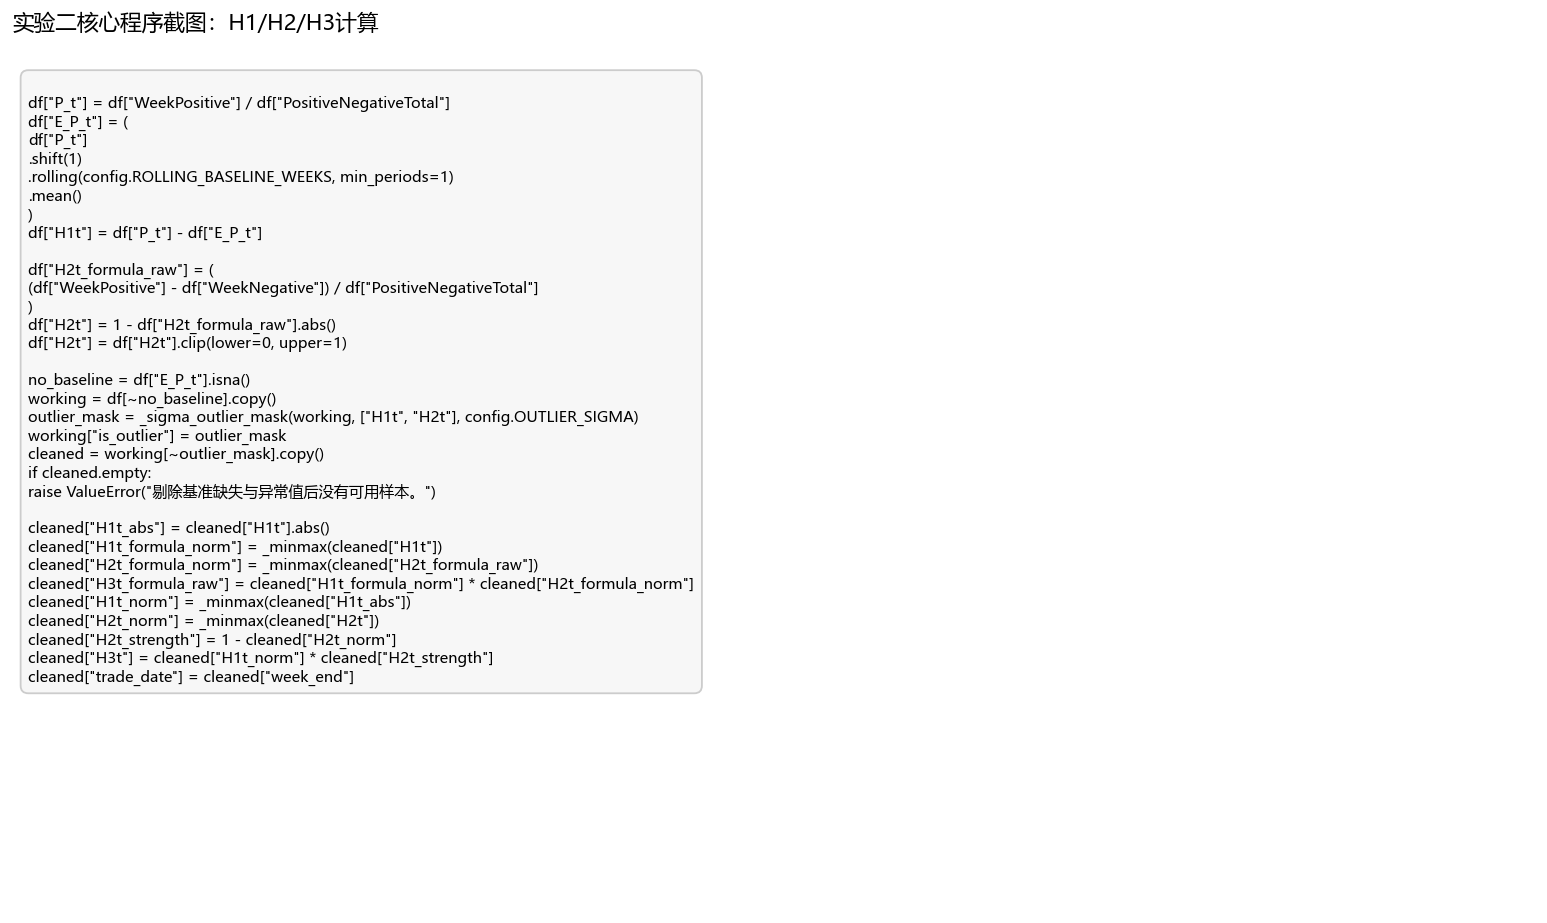
\includegraphics[width=0.96\textwidth]{core_program_snippet.png}
    \caption{系统主要程序截图：H1/H2/H3 计算}
    \label{fig:core-code}
\end{figure}

\section{结果与质量检查}

\subsection{质量检查}

\begin{table}[H]
    \centering
    \scriptsize
    \caption{实验二质量检查结果}
    \label{tab:quality-checks}
    \begin{tabular}{L{0.30\textwidth}cL{0.50\textwidth}}
        \toprule
        检查项 & 结果 & 说明 \\
        \midrule
        关键字段无缺失 & True & \texttt{trade\_date}、\texttt{H1t}、\texttt{H2t}、\texttt{H3t} 均完整 \\
        日期单调递增 & True & 输出时序按交易周末日期升序排列 \\
        $P_t$ 范围合法 & True & $P_t$ 为正面新闻占正负情绪新闻比例 \\
        $H2_t$ 范围合法 & True & $H2_t$ 为分歧度，越接近 0 表示越一边倒 \\
        任务书公式 H2 原文列范围合法 & True & \texttt{H2t\_formula\_raw} 保留公式 4 直接转写结果 \\
        $H3_t$ 范围合法 & True & $H3_t$ 由 $|H1|$ 强度和 $H2$ 反向强度相乘 \\
        \bottomrule
    \end{tabular}
\end{table}

\subsection{描述统计}

\begin{table}[H]
    \centering
    \scriptsize
    \caption{主要指标描述统计}
    \label{tab:summary-stats}
    \begin{tabular}{lrrrrrr}
        \toprule
        指标 & 样本数 & 均值 & 标准差 & 最小值 & 中位数 & 最大值 \\
        \midrule
        $P_t$ & 50 & 0.823775 & 0.058090 & 0.694444 & 0.821856 & 0.935897 \\
        $H1_t$ & 50 & -0.001593 & 0.060426 & -0.134822 & -0.010121 & 0.148983 \\
        \texttt{H2t\_formula\_raw} & 50 & 0.647551 & 0.116179 & 0.388889 & 0.643712 & 0.871795 \\
        $H2_t$ & 50 & 0.352449 & 0.116179 & 0.128205 & 0.356288 & 0.611111 \\
        $H2$ 一致性强度 & 50 & 0.535637 & 0.240583 & 0.000000 & 0.527686 & 1.000000 \\
        \texttt{H3t\_formula\_raw} & 50 & 0.479176 & 0.212511 & 0.000000 & 0.507230 & 1.000000 \\
        $H3_t$ & 50 & 0.168144 & 0.178341 & 0.000000 & 0.121895 & 0.864687 \\
        \bottomrule
    \end{tabular}
\end{table}

\subsection{羊群效应时序表}

\begin{figure}[H]
    \centering
    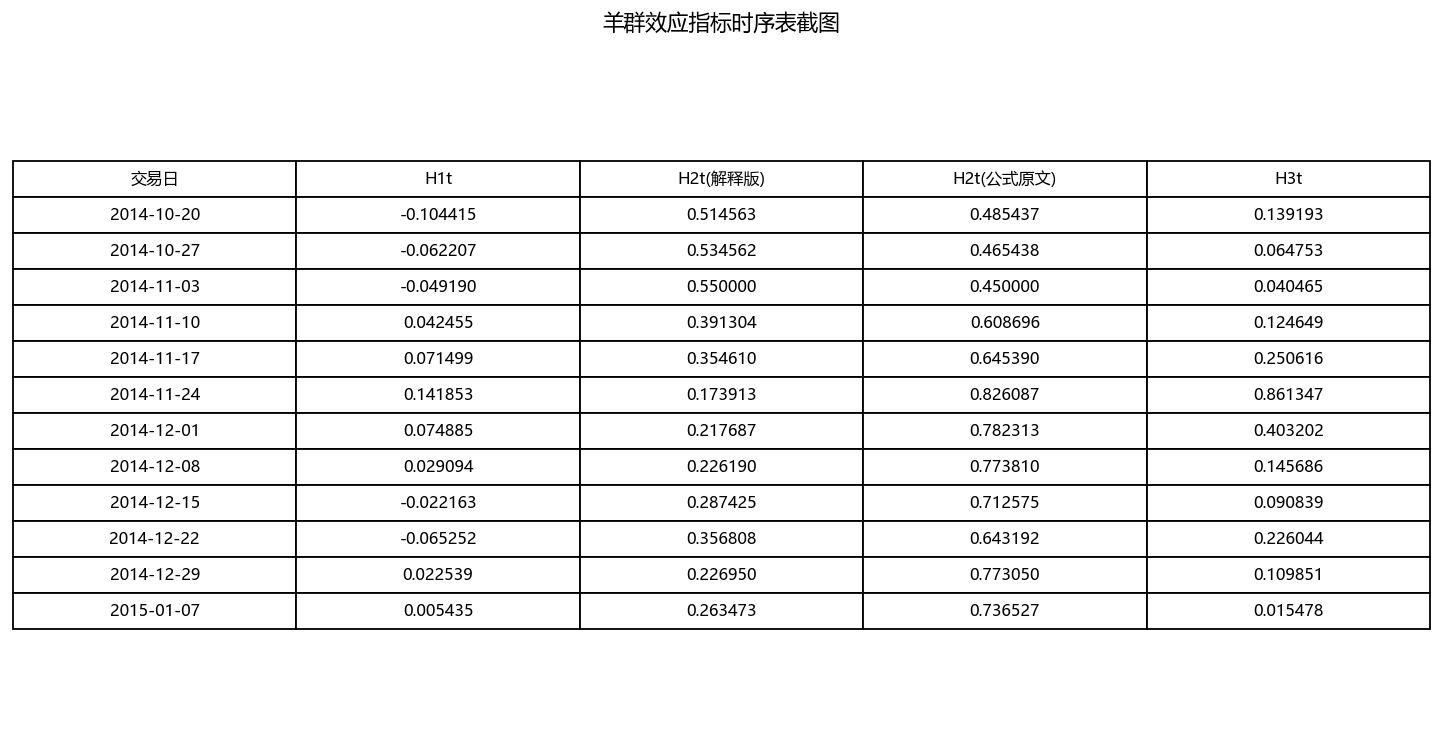
\includegraphics[width=0.98\textwidth]{weekly_herd_index_table.png}
    \caption{羊群效应指标时序表截图}
    \label{fig:herd-table}
\end{figure}

\subsection{羊群效应时序图}

\begin{figure}[H]
    \centering
    
\includegraphics[width=0.96\textwidth]{herd_index_timeseries.png}
    \caption{周度羊群效应指标时序}
    \label{fig:herd-timeseries}
\end{figure}

图 \ref{fig:herd-timeseries} 显示，$H3_t$ 并不是单纯跟随乐观占比上升，而是在情绪偏离强且观点集中时出现高值。这说明综合指标能够过滤普通情绪波动，只突出更符合羊群效应定义的交易周。

\begin{figure}[H]
    \centering
    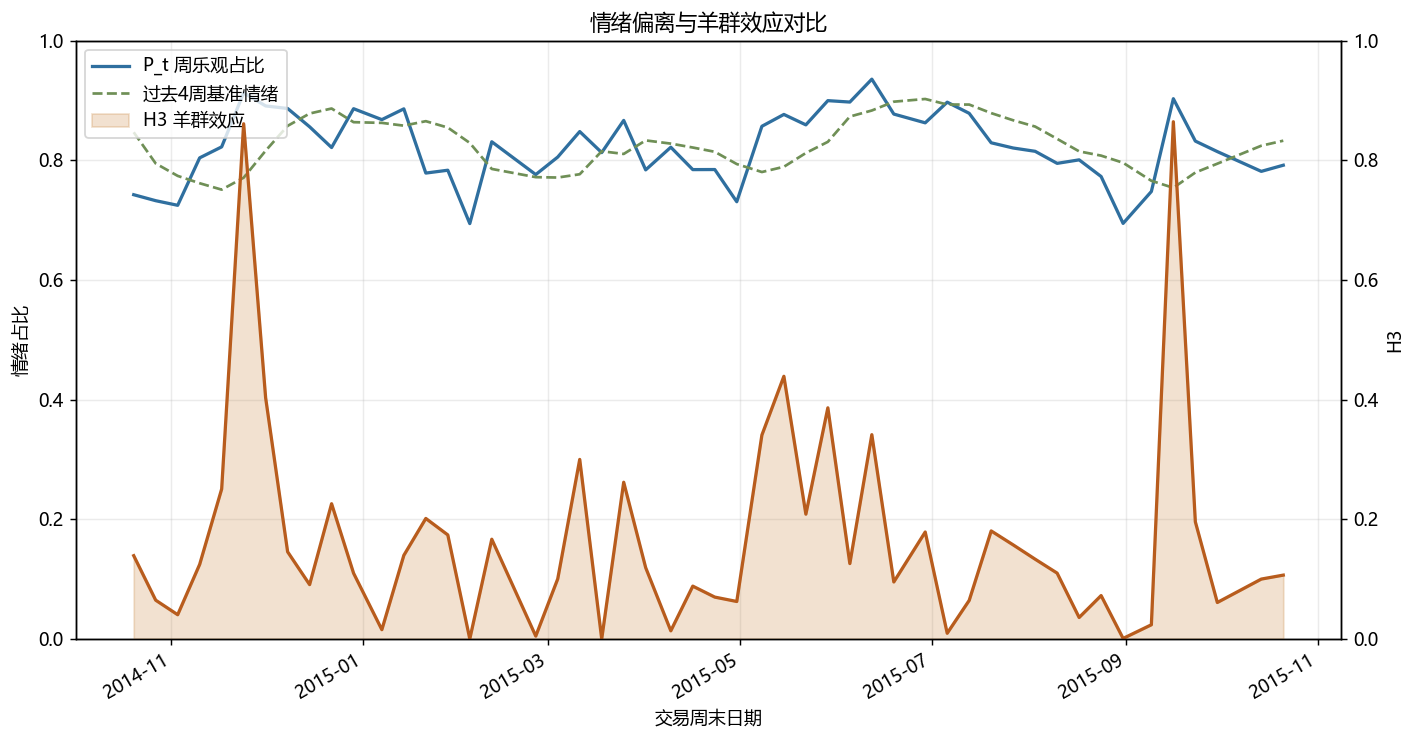
\includegraphics[width=0.96\textwidth]{sentiment_vs_herd.png}
    \caption{情绪占比与羊群效应对比}
    \label{fig:sentiment-vs-herd}
\end{figure}

\begin{figure}[H]
    \centering
    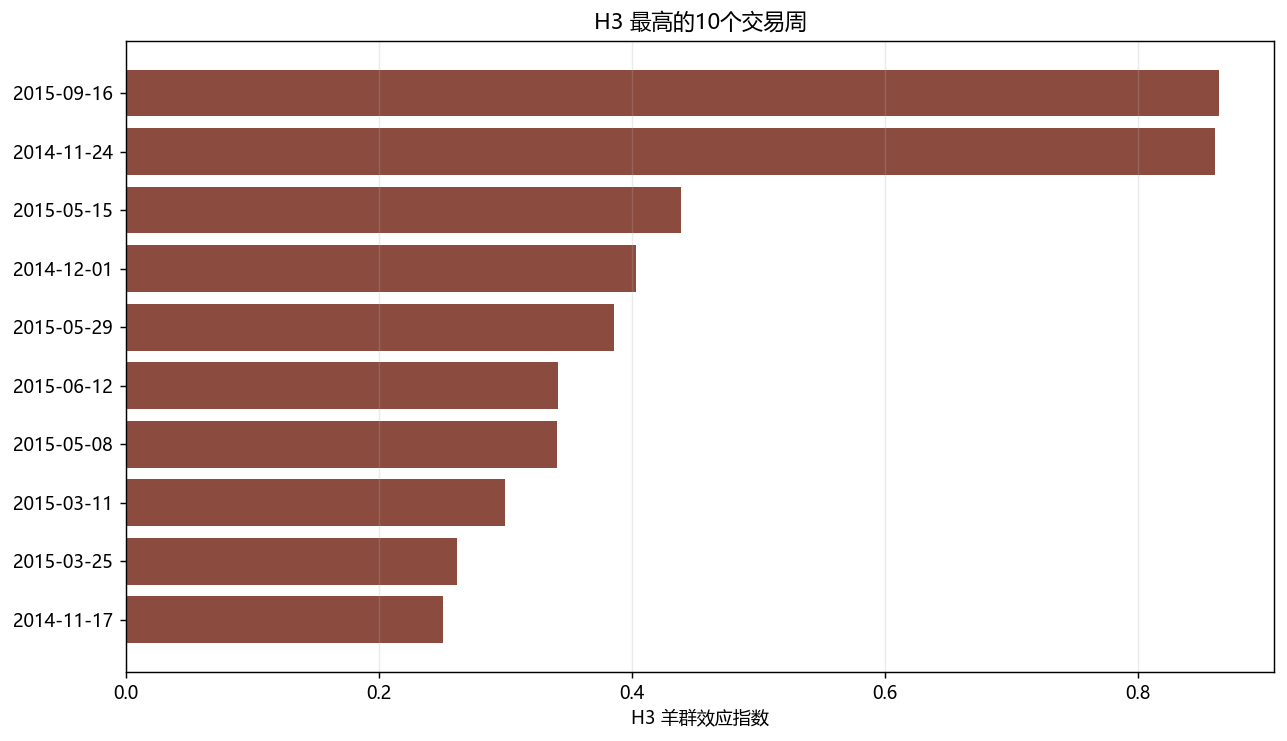
\includegraphics[width=0.88\textwidth]{top_herd_weeks.png}
    \caption{H3 最高的 10 个交易周}
    \label{fig:top-herd}
\end{figure}

\begin{figure}[H]
    \centering
    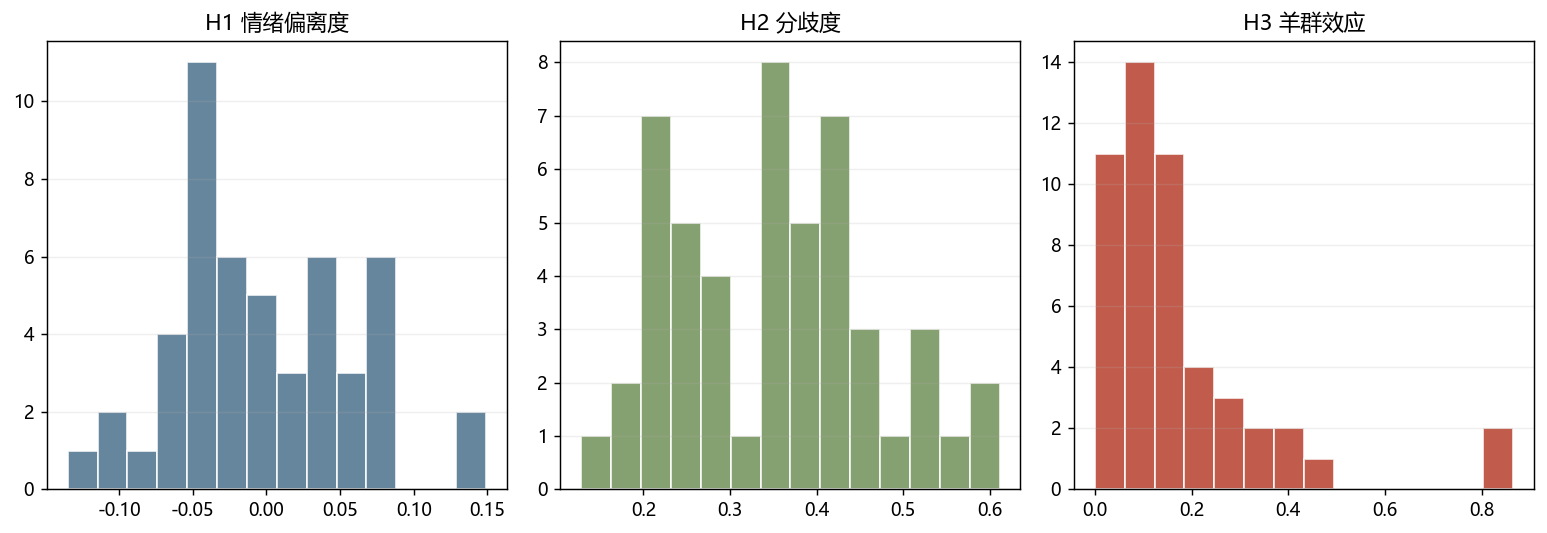
\includegraphics[width=0.92\textwidth]{indicator_distribution.png}
    \caption{H1、H2、H3 指标分布}
    \label{fig:indicator-distribution}
\end{figure}

\section{高羊群效应周分析}

\begin{table}[H]
    \centering
    \scriptsize
    \caption{H3 排名前 10 的交易周}
    \label{tab:top-herd-weeks}
    \begin{tabular}{rlrrrrrrr}
        \toprule
        排名 & 交易日 & $P_t$ & $E(P_t)$ & $H1_t$ & $H2_t$ & $H2^{raw}_t$ & $H3_t$ & 新闻数 \\
        \midrule
        1 & 2015-09-16 & 0.903226 & 0.754243 & 0.148983 & 0.193548 & 0.806452 & 0.864687 & 553 \\
        2 & 2014-11-24 & 0.913043 & 0.771190 & 0.141853 & 0.173913 & 0.826087 & 0.861347 & 640 \\
        3 & 2015-05-15 & 0.876923 & 0.789402 & 0.087521 & 0.246154 & 0.753846 & 0.439126 & 594 \\
        4 & 2014-12-01 & 0.891156 & 0.816272 & 0.074885 & 0.217687 & 0.782313 & 0.403202 & 620 \\
        5 & 2015-05-29 & 0.900000 & 0.831134 & 0.068866 & 0.200000 & 0.800000 & 0.386402 & 568 \\
        6 & 2015-06-12 & 0.935897 & 0.883516 & 0.052381 & 0.128205 & 0.871795 & 0.341510 & 687 \\
        7 & 2015-05-08 & 0.857143 & 0.780645 & 0.076498 & 0.285714 & 0.714286 & 0.340894 & 586 \\
        8 & 2015-03-11 & 0.848315 & 0.776945 & 0.071370 & 0.303371 & 0.696629 & 0.300119 & 534 \\
        9 & 2015-03-25 & 0.866953 & 0.810883 & 0.056070 & 0.266094 & 0.733906 & 0.261961 & 586 \\
        10 & 2014-11-17 & 0.822695 & 0.751196 & 0.071499 & 0.354610 & 0.645390 & 0.250616 & 588 \\
        \bottomrule
    \end{tabular}
\end{table}

最高羊群效应周为 2015-09-16。当周 $P_t=0.903226$，明显高于过去 4 周基准 $0.754243$，$H1_t=0.148983$；同时 $H2_t=0.193548$，说明正负观点较为单边。情绪异常和观点集中两个条件同时满足，因此 $H3_t$ 达到 0.864687。

\section{数据库与文件输出}

本实验输出的核心文件如下：

\begin{itemize}
    \item \path{outputs/experiment2/weekly_herd_index.csv}：实验二核心羊群指标表。
    \item \path{outputs/experiment2/experiment2.db}：SQLite 数据库，包含输入、指标、质量检查、描述统计和高羊群周表。
    \item \path{outputs/experiment2/quality_checks.csv}：质量检查结果。
    \item \path{outputs/experiment2/summary_statistics.csv}：描述统计表。
    \item \path{outputs/experiment2/top_herd_weeks.csv}：H3 最高的 10 个交易周。
    \item AI 交互记录与 AI 代码审查表：位于 \path{outputs/experiment2/}，文件名为中文 Markdown。
    \item 实验二代码附录：位于 \path{outputs/experiment2/}，文件名为中文 Markdown。
\end{itemize}

\section{金融逻辑与合理性说明}

羊群效应并不等于市场乐观，也不等于市场悲观。只有当情绪相对历史基准发生显著偏离，并且投资者观点呈现单边集中时，才更接近羊群行为。$H1_t$ 捕捉“本周是否反常”，$H2_t$ 捕捉“本周是否一边倒”，$H3_t$ 将两者合成，因此能够降低普通情绪波动或多空分歧周对指标的干扰。

本实验同时保留公式原文转写列和解释一致版最终指标，是因为指导书的公式文本与文字解释存在方向上的差异。保留两套口径可以提高审查透明度：如果按公式原文检查，可以查看 \texttt{H2t\_formula\_raw} 和 \texttt{H3t\_formula\_raw}；如果按“情绪反常且观点一边倒”的金融含义分析，则使用最终输出的 \texttt{H2t} 与 \texttt{H3t}。

\section{结论}

实验二已完成从周度情绪指标到羊群效应指数的完整构建流程。结果表明，样本期内羊群效应高值主要出现在正面情绪占比显著高于历史基准且正负观点较单边的交易周。输出的 \texttt{weekly\_herd\_index.csv} 具备完整交易日、$H1_t$、$H2_t$、$H3_t$ 字段，可直接作为实验三回归和机器学习建模的输入。

\end{document}
